%!TEX program=xelatex
\documentclass[UTF8]{ctexart}

%%%%%% 导入包 %%%%%%
\usepackage{graphicx}
\usepackage{float}
\usepackage{xcolor}
\usepackage{algorithm,algorithmicx}
\usepackage{algpseudocode}
\usepackage{amsmath,amssymb,amsthm}

%%%%%% 算法部分改为中文显示 %%%%%%%%%
\floatname{algorithm}{算法}
\renewcommand{\algorithmicrequire}{\textbf{输入:}}
\renewcommand{\algorithmicensure}{\textbf{输出:}}

%%%% 正文开始 %%%%
\begin{document}

\title{第一次作业}

\author{陈文宇}

\date{\today}

\maketitle{}

为了便于输出步长、精度和收敛阶情况,我选择了这样分划,\\
对于n = 100:100:1000,$$h=\dfrac{right-left}{n}$$

利用复化Simpson公式,求解区间(left,right)上函数的数值积分,并求解精度和误差
$$r=| \frac{I-I_{n}(f)}{I}|, R = I-I_{n}(f)$$

具体结果如下表及图片展示,可得复化复化Simpson公式的收敛阶为4阶。


\newpage
% Table generated by Excel2LaTeX from sheet 'Sheet1'
\begin{table*}[htbp]
	\centering
	\caption{xsin(x)的步长与精度}
	\scalebox{0.75}{
	\begin{tabular}{|r|r|r|r|r|r|r|r|r|r|r|}
		\hline	
		h & 6.28E-02 & 3.14E-02 & 2.09E-02 & 1.57E-02 & 1.26E-02 & 1.05E-02 & 8.98E-03 & 7.85E-03 & 6.98E-03 & 6.28E-03 \\
		\hline	
		r & 8.66E-08 & 5.41E-09 & 1.07E-09 & 3.38E-10 & 1.39E-10 & 6.68E-11 & 3.61E-11 & 2.11E-11 & 1.32E-11 & 8.66E-12 \\
		\hline	
	\end{tabular}%

	}
\end{table*}%

\begin{figure}[H]
	\centering
	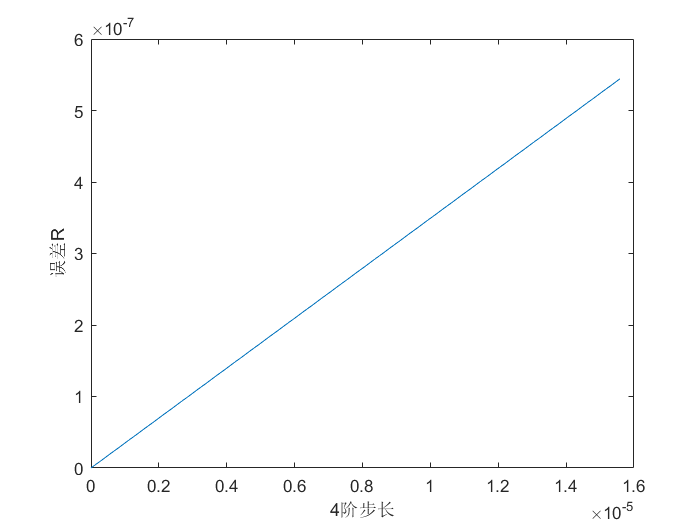
\includegraphics[scale=0.7]{xsinx_H_R_.png}
	\caption{xsinx的4阶步长和误差关系图}
\end{figure}

\newpage 

% Table generated by Excel2LaTeX from sheet 'Sheet1'
\begin{table*}[htbp]
	\centering
	\caption{$\sqrt{x}$的步长与精度}
	\scalebox{0.8}{
	\begin{tabular}{|r|r|r|r|r|r|r|r|r|r|}
		\hline	
		h & 5.00E-03 & 3.33E-03 & 2.50E-03 & 2.00E-03 & 1.67E-03 & 1.43E-03 & 1.25E-03 & 1.11E-03 & 1.00E-03 \\
		\hline	
		r & 6.67E-01 & 6.67E-01 & 6.67E-01 & 6.67E-01 & 6.67E-01 & 6.67E-01 & 6.67E-01 & 6.67E-01 & 6.67E-01 \\
		\hline	
	\end{tabular}%

	}
\end{table*}%


\begin{figure}[H]
	\centering
	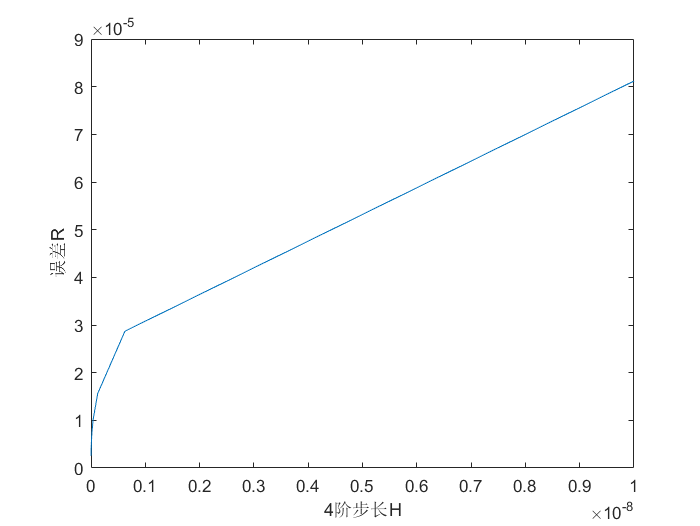
\includegraphics[scale=0.7]{sqrtx_H_R_.png}
	\caption{$\sqrt{x}$的4阶步长和误差关系图}
\end{figure}


\end{document}
